\documentclass[11pt]{article}

    \usepackage[breakable]{tcolorbox}
    \usepackage{parskip} % Stop auto-indenting (to mimic markdown behaviour)
    

    % Basic figure setup, for now with no caption control since it's done
    % automatically by Pandoc (which extracts ![](path) syntax from Markdown).
    \usepackage{graphicx}
    % Maintain compatibility with old templates. Remove in nbconvert 6.0
    \let\Oldincludegraphics\includegraphics
    % Ensure that by default, figures have no caption (until we provide a
    % proper Figure object with a Caption API and a way to capture that
    % in the conversion process - todo).
    \usepackage{caption}
    %\DeclareCaptionFormat{nocaption}{}
    %\captionsetup{format=nocaption,aboveskip=0pt,belowskip=0pt}

    \usepackage{float}
    \floatplacement{figure}{H} % forces figures to be placed at the correct location
    \usepackage{xcolor} % Allow colors to be defined
    \usepackage{enumerate} % Needed for markdown enumerations to work
    \usepackage{geometry} % Used to adjust the document margins
    \usepackage{amsmath} % Equations
    \usepackage{amssymb} % Equations
    \usepackage{textcomp} % defines textquotesingle
    % Hack from http://tex.stackexchange.com/a/47451/13684:
    \AtBeginDocument{%
        \def\PYZsq{\textquotesingle}% Upright quotes in Pygmentized code
    }
    \usepackage{upquote} % Upright quotes for verbatim code
    \usepackage{eurosym} % defines \euro

    \usepackage{iftex}
    \ifPDFTeX
        \usepackage[T1]{fontenc}
        \IfFileExists{alphabeta.sty}{
              \usepackage{alphabeta}
          }{
              \usepackage[mathletters]{ucs}
              \usepackage[utf8x]{inputenc}
          }
    \else
        \usepackage{fontspec}
        \usepackage{unicode-math}
    \fi

    \usepackage{fancyvrb} % verbatim replacement that allows latex
    \usepackage{grffile} % extends the file name processing of package graphics 
                         % to support a larger range
    \makeatletter % fix for old versions of grffile with XeLaTeX
    \@ifpackagelater{grffile}{2019/11/01}
    {
      % Do nothing on new versions
    }
    {
      \def\Gread@@xetex#1{%
        \IfFileExists{"\Gin@base".bb}%
        {\Gread@eps{\Gin@base.bb}}%
        {\Gread@@xetex@aux#1}%
      }
    }
    \makeatother
    \usepackage[Export]{adjustbox} % Used to constrain images to a maximum size
    \adjustboxset{max size={0.9\linewidth}{0.9\paperheight}}

    % The hyperref package gives us a pdf with properly built
    % internal navigation ('pdf bookmarks' for the table of contents,
    % internal cross-reference links, web links for URLs, etc.)
    \usepackage{hyperref}
    % The default LaTeX title has an obnoxious amount of whitespace. By default,
    % titling removes some of it. It also provides customization options.
    \usepackage{titling}
    \usepackage{longtable} % longtable support required by pandoc >1.10
    \usepackage{booktabs}  % table support for pandoc > 1.12.2
    \usepackage{array}     % table support for pandoc >= 2.11.3
    \usepackage{calc}      % table minipage width calculation for pandoc >= 2.11.1
    \usepackage[inline]{enumitem} % IRkernel/repr support (it uses the enumerate* environment)
    \usepackage[normalem]{ulem} % ulem is needed to support strikethroughs (\sout)
                                % normalem makes italics be italics, not underlines
    \usepackage{mathrsfs}
    \usepackage{listings}
    \usepackage{xcolor}

    \definecolor{codegreen}{rgb}{0,0.6,0}
    \definecolor{codegray}{rgb}{0.5,0.5,0.5}
    \definecolor{codepurple}{rgb}{0.58,0,0.82}
    \definecolor{backcolour}{rgb}{0.95,0.95,0.92}
    
    \lstdefinestyle{mystyle}{
        backgroundcolor=\color{backcolour},   
        commentstyle=\color{codegreen},
        keywordstyle=\color{magenta},
        numberstyle=\tiny\color{codegray},
        stringstyle=\color{codepurple},
        basicstyle=\ttfamily\footnotesize,
        breakatwhitespace=false,         
        breaklines=true,                 
        captionpos=b,                    
        keepspaces=true,                 
        numbers=left,                    
        numbersep=5pt,                  
        showspaces=false,                
        showstringspaces=false,
        showtabs=false,                  
        tabsize=2
    }
    
    \lstset{style=mystyle}

    % Colors for the hyperref package
    \definecolor{urlcolor}{rgb}{0,.145,.698}
    \definecolor{linkcolor}{rgb}{0,.145,.698}
    \definecolor{citecolor}{rgb}{.12,.54,.11}

    % ANSI colors
    \definecolor{ansi-black}{HTML}{3E424D}
    \definecolor{ansi-black-intense}{HTML}{282C36}
    \definecolor{ansi-red}{HTML}{E75C58}
    \definecolor{ansi-red-intense}{HTML}{B22B31}
    \definecolor{ansi-green}{HTML}{00A250}
    \definecolor{ansi-green-intense}{HTML}{007427}
    \definecolor{ansi-yellow}{HTML}{DDB62B}
    \definecolor{ansi-yellow-intense}{HTML}{B27D12}
    \definecolor{ansi-blue}{HTML}{208FFB}
    \definecolor{ansi-blue-intense}{HTML}{0065CA}
    \definecolor{ansi-magenta}{HTML}{D160C4}
    \definecolor{ansi-magenta-intense}{HTML}{A03196}
    \definecolor{ansi-cyan}{HTML}{60C6C8}
    \definecolor{ansi-cyan-intense}{HTML}{258F8F}
    \definecolor{ansi-white}{HTML}{C5C1B4}
    \definecolor{ansi-white-intense}{HTML}{A1A6B2}
    \definecolor{ansi-default-inverse-fg}{HTML}{FFFFFF}
    \definecolor{ansi-default-inverse-bg}{HTML}{000000}

    % common color for the border for error outputs.
    \definecolor{outerrorbackground}{HTML}{FFDFDF}

    % commands and environments needed by pandoc snippets
    % extracted from the output of `pandoc -s`
    \providecommand{\tightlist}{%
      \setlength{\itemsep}{0pt}\setlength{\parskip}{0pt}}
    \DefineVerbatimEnvironment{Highlighting}{Verbatim}{commandchars=\\\{\}}
    % Add ',fontsize=\small' for more characters per line
    \newenvironment{Shaded}{}{}
    \newcommand{\KeywordTok}[1]{\textcolor[rgb]{0.00,0.44,0.13}{\textbf{{#1}}}}
    \newcommand{\DataTypeTok}[1]{\textcolor[rgb]{0.56,0.13,0.00}{{#1}}}
    \newcommand{\DecValTok}[1]{\textcolor[rgb]{0.25,0.63,0.44}{{#1}}}
    \newcommand{\BaseNTok}[1]{\textcolor[rgb]{0.25,0.63,0.44}{{#1}}}
    \newcommand{\FloatTok}[1]{\textcolor[rgb]{0.25,0.63,0.44}{{#1}}}
    \newcommand{\CharTok}[1]{\textcolor[rgb]{0.25,0.44,0.63}{{#1}}}
    \newcommand{\StringTok}[1]{\textcolor[rgb]{0.25,0.44,0.63}{{#1}}}
    \newcommand{\CommentTok}[1]{\textcolor[rgb]{0.38,0.63,0.69}{\textit{{#1}}}}
    \newcommand{\OtherTok}[1]{\textcolor[rgb]{0.00,0.44,0.13}{{#1}}}
    \newcommand{\AlertTok}[1]{\textcolor[rgb]{1.00,0.00,0.00}{\textbf{{#1}}}}
    \newcommand{\FunctionTok}[1]{\textcolor[rgb]{0.02,0.16,0.49}{{#1}}}
    \newcommand{\RegionMarkerTok}[1]{{#1}}
    \newcommand{\ErrorTok}[1]{\textcolor[rgb]{1.00,0.00,0.00}{\textbf{{#1}}}}
    \newcommand{\NormalTok}[1]{{#1}}
    
    % Additional commands for more recent versions of Pandoc
    \newcommand{\ConstantTok}[1]{\textcolor[rgb]{0.53,0.00,0.00}{{#1}}}
    \newcommand{\SpecialCharTok}[1]{\textcolor[rgb]{0.25,0.44,0.63}{{#1}}}
    \newcommand{\VerbatimStringTok}[1]{\textcolor[rgb]{0.25,0.44,0.63}{{#1}}}
    \newcommand{\SpecialStringTok}[1]{\textcolor[rgb]{0.73,0.40,0.53}{{#1}}}
    \newcommand{\ImportTok}[1]{{#1}}
    \newcommand{\DocumentationTok}[1]{\textcolor[rgb]{0.73,0.13,0.13}{\textit{{#1}}}}
    \newcommand{\AnnotationTok}[1]{\textcolor[rgb]{0.38,0.63,0.69}{\textbf{\textit{{#1}}}}}
    \newcommand{\CommentVarTok}[1]{\textcolor[rgb]{0.38,0.63,0.69}{\textbf{\textit{{#1}}}}}
    \newcommand{\VariableTok}[1]{\textcolor[rgb]{0.10,0.09,0.49}{{#1}}}
    \newcommand{\ControlFlowTok}[1]{\textcolor[rgb]{0.00,0.44,0.13}{\textbf{{#1}}}}
    \newcommand{\OperatorTok}[1]{\textcolor[rgb]{0.40,0.40,0.40}{{#1}}}
    \newcommand{\BuiltInTok}[1]{{#1}}
    \newcommand{\ExtensionTok}[1]{{#1}}
    \newcommand{\PreprocessorTok}[1]{\textcolor[rgb]{0.74,0.48,0.00}{{#1}}}
    \newcommand{\AttributeTok}[1]{\textcolor[rgb]{0.49,0.56,0.16}{{#1}}}
    \newcommand{\InformationTok}[1]{\textcolor[rgb]{0.38,0.63,0.69}{\textbf{\textit{{#1}}}}}
    \newcommand{\WarningTok}[1]{\textcolor[rgb]{0.38,0.63,0.69}{\textbf{\textit{{#1}}}}}
    
    
    % Define a nice break command that doesn't care if a line doesn't already
    % exist.
    \def\br{\hspace*{\fill} \\* }
    % Math Jax compatibility definitions
    \def\gt{>}
    \def\lt{<}
    \let\Oldtex\TeX
    \let\Oldlatex\LaTeX
    \renewcommand{\TeX}{\textrm{\Oldtex}}
    \renewcommand{\LaTeX}{\textrm{\Oldlatex}}
    % Document parameters
    % Document title
    \title{PEC 3}
    
    
    
    
    
% Pygments definitions
\makeatletter
\def\PY@reset{\let\PY@it=\relax \let\PY@bf=\relax%
    \let\PY@ul=\relax \let\PY@tc=\relax%
    \let\PY@bc=\relax \let\PY@ff=\relax}
\def\PY@tok#1{\csname PY@tok@#1\endcsname}
\def\PY@toks#1+{\ifx\relax#1\empty\else%
    \PY@tok{#1}\expandafter\PY@toks\fi}
\def\PY@do#1{\PY@bc{\PY@tc{\PY@ul{%
    \PY@it{\PY@bf{\PY@ff{#1}}}}}}}
\def\PY#1#2{\PY@reset\PY@toks#1+\relax+\PY@do{#2}}

\@namedef{PY@tok@w}{\def\PY@tc##1{\textcolor[rgb]{0.73,0.73,0.73}{##1}}}
\@namedef{PY@tok@c}{\let\PY@it=\textit\def\PY@tc##1{\textcolor[rgb]{0.24,0.48,0.48}{##1}}}
\@namedef{PY@tok@cp}{\def\PY@tc##1{\textcolor[rgb]{0.61,0.40,0.00}{##1}}}
\@namedef{PY@tok@k}{\let\PY@bf=\textbf\def\PY@tc##1{\textcolor[rgb]{0.00,0.50,0.00}{##1}}}
\@namedef{PY@tok@kp}{\def\PY@tc##1{\textcolor[rgb]{0.00,0.50,0.00}{##1}}}
\@namedef{PY@tok@kt}{\def\PY@tc##1{\textcolor[rgb]{0.69,0.00,0.25}{##1}}}
\@namedef{PY@tok@o}{\def\PY@tc##1{\textcolor[rgb]{0.40,0.40,0.40}{##1}}}
\@namedef{PY@tok@ow}{\let\PY@bf=\textbf\def\PY@tc##1{\textcolor[rgb]{0.67,0.13,1.00}{##1}}}
\@namedef{PY@tok@nb}{\def\PY@tc##1{\textcolor[rgb]{0.00,0.50,0.00}{##1}}}
\@namedef{PY@tok@nf}{\def\PY@tc##1{\textcolor[rgb]{0.00,0.00,1.00}{##1}}}
\@namedef{PY@tok@nc}{\let\PY@bf=\textbf\def\PY@tc##1{\textcolor[rgb]{0.00,0.00,1.00}{##1}}}
\@namedef{PY@tok@nn}{\let\PY@bf=\textbf\def\PY@tc##1{\textcolor[rgb]{0.00,0.00,1.00}{##1}}}
\@namedef{PY@tok@ne}{\let\PY@bf=\textbf\def\PY@tc##1{\textcolor[rgb]{0.80,0.25,0.22}{##1}}}
\@namedef{PY@tok@nv}{\def\PY@tc##1{\textcolor[rgb]{0.10,0.09,0.49}{##1}}}
\@namedef{PY@tok@no}{\def\PY@tc##1{\textcolor[rgb]{0.53,0.00,0.00}{##1}}}
\@namedef{PY@tok@nl}{\def\PY@tc##1{\textcolor[rgb]{0.46,0.46,0.00}{##1}}}
\@namedef{PY@tok@ni}{\let\PY@bf=\textbf\def\PY@tc##1{\textcolor[rgb]{0.44,0.44,0.44}{##1}}}
\@namedef{PY@tok@na}{\def\PY@tc##1{\textcolor[rgb]{0.41,0.47,0.13}{##1}}}
\@namedef{PY@tok@nt}{\let\PY@bf=\textbf\def\PY@tc##1{\textcolor[rgb]{0.00,0.50,0.00}{##1}}}
\@namedef{PY@tok@nd}{\def\PY@tc##1{\textcolor[rgb]{0.67,0.13,1.00}{##1}}}
\@namedef{PY@tok@s}{\def\PY@tc##1{\textcolor[rgb]{0.73,0.13,0.13}{##1}}}
\@namedef{PY@tok@sd}{\let\PY@it=\textit\def\PY@tc##1{\textcolor[rgb]{0.73,0.13,0.13}{##1}}}
\@namedef{PY@tok@si}{\let\PY@bf=\textbf\def\PY@tc##1{\textcolor[rgb]{0.64,0.35,0.47}{##1}}}
\@namedef{PY@tok@se}{\let\PY@bf=\textbf\def\PY@tc##1{\textcolor[rgb]{0.67,0.36,0.12}{##1}}}
\@namedef{PY@tok@sr}{\def\PY@tc##1{\textcolor[rgb]{0.64,0.35,0.47}{##1}}}
\@namedef{PY@tok@ss}{\def\PY@tc##1{\textcolor[rgb]{0.10,0.09,0.49}{##1}}}
\@namedef{PY@tok@sx}{\def\PY@tc##1{\textcolor[rgb]{0.00,0.50,0.00}{##1}}}
\@namedef{PY@tok@m}{\def\PY@tc##1{\textcolor[rgb]{0.40,0.40,0.40}{##1}}}
\@namedef{PY@tok@gh}{\let\PY@bf=\textbf\def\PY@tc##1{\textcolor[rgb]{0.00,0.00,0.50}{##1}}}
\@namedef{PY@tok@gu}{\let\PY@bf=\textbf\def\PY@tc##1{\textcolor[rgb]{0.50,0.00,0.50}{##1}}}
\@namedef{PY@tok@gd}{\def\PY@tc##1{\textcolor[rgb]{0.63,0.00,0.00}{##1}}}
\@namedef{PY@tok@gi}{\def\PY@tc##1{\textcolor[rgb]{0.00,0.52,0.00}{##1}}}
\@namedef{PY@tok@gr}{\def\PY@tc##1{\textcolor[rgb]{0.89,0.00,0.00}{##1}}}
\@namedef{PY@tok@ge}{\let\PY@it=\textit}
\@namedef{PY@tok@gs}{\let\PY@bf=\textbf}
\@namedef{PY@tok@gp}{\let\PY@bf=\textbf\def\PY@tc##1{\textcolor[rgb]{0.00,0.00,0.50}{##1}}}
\@namedef{PY@tok@go}{\def\PY@tc##1{\textcolor[rgb]{0.44,0.44,0.44}{##1}}}
\@namedef{PY@tok@gt}{\def\PY@tc##1{\textcolor[rgb]{0.00,0.27,0.87}{##1}}}
\@namedef{PY@tok@err}{\def\PY@bc##1{{\setlength{\fboxsep}{\string -\fboxrule}\fcolorbox[rgb]{1.00,0.00,0.00}{1,1,1}{\strut ##1}}}}
\@namedef{PY@tok@kc}{\let\PY@bf=\textbf\def\PY@tc##1{\textcolor[rgb]{0.00,0.50,0.00}{##1}}}
\@namedef{PY@tok@kd}{\let\PY@bf=\textbf\def\PY@tc##1{\textcolor[rgb]{0.00,0.50,0.00}{##1}}}
\@namedef{PY@tok@kn}{\let\PY@bf=\textbf\def\PY@tc##1{\textcolor[rgb]{0.00,0.50,0.00}{##1}}}
\@namedef{PY@tok@kr}{\let\PY@bf=\textbf\def\PY@tc##1{\textcolor[rgb]{0.00,0.50,0.00}{##1}}}
\@namedef{PY@tok@bp}{\def\PY@tc##1{\textcolor[rgb]{0.00,0.50,0.00}{##1}}}
\@namedef{PY@tok@fm}{\def\PY@tc##1{\textcolor[rgb]{0.00,0.00,1.00}{##1}}}
\@namedef{PY@tok@vc}{\def\PY@tc##1{\textcolor[rgb]{0.10,0.09,0.49}{##1}}}
\@namedef{PY@tok@vg}{\def\PY@tc##1{\textcolor[rgb]{0.10,0.09,0.49}{##1}}}
\@namedef{PY@tok@vi}{\def\PY@tc##1{\textcolor[rgb]{0.10,0.09,0.49}{##1}}}
\@namedef{PY@tok@vm}{\def\PY@tc##1{\textcolor[rgb]{0.10,0.09,0.49}{##1}}}
\@namedef{PY@tok@sa}{\def\PY@tc##1{\textcolor[rgb]{0.73,0.13,0.13}{##1}}}
\@namedef{PY@tok@sb}{\def\PY@tc##1{\textcolor[rgb]{0.73,0.13,0.13}{##1}}}
\@namedef{PY@tok@sc}{\def\PY@tc##1{\textcolor[rgb]{0.73,0.13,0.13}{##1}}}
\@namedef{PY@tok@dl}{\def\PY@tc##1{\textcolor[rgb]{0.73,0.13,0.13}{##1}}}
\@namedef{PY@tok@s2}{\def\PY@tc##1{\textcolor[rgb]{0.73,0.13,0.13}{##1}}}
\@namedef{PY@tok@sh}{\def\PY@tc##1{\textcolor[rgb]{0.73,0.13,0.13}{##1}}}
\@namedef{PY@tok@s1}{\def\PY@tc##1{\textcolor[rgb]{0.73,0.13,0.13}{##1}}}
\@namedef{PY@tok@mb}{\def\PY@tc##1{\textcolor[rgb]{0.40,0.40,0.40}{##1}}}
\@namedef{PY@tok@mf}{\def\PY@tc##1{\textcolor[rgb]{0.40,0.40,0.40}{##1}}}
\@namedef{PY@tok@mh}{\def\PY@tc##1{\textcolor[rgb]{0.40,0.40,0.40}{##1}}}
\@namedef{PY@tok@mi}{\def\PY@tc##1{\textcolor[rgb]{0.40,0.40,0.40}{##1}}}
\@namedef{PY@tok@il}{\def\PY@tc##1{\textcolor[rgb]{0.40,0.40,0.40}{##1}}}
\@namedef{PY@tok@mo}{\def\PY@tc##1{\textcolor[rgb]{0.40,0.40,0.40}{##1}}}
\@namedef{PY@tok@ch}{\let\PY@it=\textit\def\PY@tc##1{\textcolor[rgb]{0.24,0.48,0.48}{##1}}}
\@namedef{PY@tok@cm}{\let\PY@it=\textit\def\PY@tc##1{\textcolor[rgb]{0.24,0.48,0.48}{##1}}}
\@namedef{PY@tok@cpf}{\let\PY@it=\textit\def\PY@tc##1{\textcolor[rgb]{0.24,0.48,0.48}{##1}}}
\@namedef{PY@tok@c1}{\let\PY@it=\textit\def\PY@tc##1{\textcolor[rgb]{0.24,0.48,0.48}{##1}}}
\@namedef{PY@tok@cs}{\let\PY@it=\textit\def\PY@tc##1{\textcolor[rgb]{0.24,0.48,0.48}{##1}}}

\def\PYZbs{\char`\\}
\def\PYZus{\char`\_}
\def\PYZob{\char`\{}
\def\PYZcb{\char`\}}
\def\PYZca{\char`\^}
\def\PYZam{\char`\&}
\def\PYZlt{\char`\<}
\def\PYZgt{\char`\>}
\def\PYZsh{\char`\#}
\def\PYZpc{\char`\%}
\def\PYZdl{\char`\$}
\def\PYZhy{\char`\-}
\def\PYZsq{\char`\'}
\def\PYZdq{\char`\"}
\def\PYZti{\char`\~}
% for compatibility with earlier versions
\def\PYZat{@}
\def\PYZlb{[}
\def\PYZrb{]}
\makeatother


    % For linebreaks inside Verbatim environment from package fancyvrb. 
    \makeatletter
        \newbox\Wrappedcontinuationbox 
        \newbox\Wrappedvisiblespacebox 
        \newcommand*\Wrappedvisiblespace {\textcolor{red}{\textvisiblespace}} 
        \newcommand*\Wrappedcontinuationsymbol {\textcolor{red}{\llap{\tiny$\m@th\hookrightarrow$}}} 
        \newcommand*\Wrappedcontinuationindent {3ex } 
        \newcommand*\Wrappedafterbreak {\kern\Wrappedcontinuationindent\copy\Wrappedcontinuationbox} 
        % Take advantage of the already applied Pygments mark-up to insert 
        % potential linebreaks for TeX processing. 
        %        {, <, #, %, $, ' and ": go to next line. 
        %        _, }, ^, &, >, - and ~: stay at end of broken line. 
        % Use of \textquotesingle for straight quote. 
        \newcommand*\Wrappedbreaksatspecials {% 
            \def\PYGZus{\discretionary{\char`\_}{\Wrappedafterbreak}{\char`\_}}% 
            \def\PYGZob{\discretionary{}{\Wrappedafterbreak\char`\{}{\char`\{}}% 
            \def\PYGZcb{\discretionary{\char`\}}{\Wrappedafterbreak}{\char`\}}}% 
            \def\PYGZca{\discretionary{\char`\^}{\Wrappedafterbreak}{\char`\^}}% 
            \def\PYGZam{\discretionary{\char`\&}{\Wrappedafterbreak}{\char`\&}}% 
            \def\PYGZlt{\discretionary{}{\Wrappedafterbreak\char`\<}{\char`\<}}% 
            \def\PYGZgt{\discretionary{\char`\>}{\Wrappedafterbreak}{\char`\>}}% 
            \def\PYGZsh{\discretionary{}{\Wrappedafterbreak\char`\#}{\char`\#}}% 
            \def\PYGZpc{\discretionary{}{\Wrappedafterbreak\char`\%}{\char`\%}}% 
            \def\PYGZdl{\discretionary{}{\Wrappedafterbreak\char`\$}{\char`\$}}% 
            \def\PYGZhy{\discretionary{\char`\-}{\Wrappedafterbreak}{\char`\-}}% 
            \def\PYGZsq{\discretionary{}{\Wrappedafterbreak\textquotesingle}{\textquotesingle}}% 
            \def\PYGZdq{\discretionary{}{\Wrappedafterbreak\char`\"}{\char`\"}}% 
            \def\PYGZti{\discretionary{\char`\~}{\Wrappedafterbreak}{\char`\~}}% 
        } 
        % Some characters . , ; ? ! / are not pygmentized. 
        % This macro makes them "active" and they will insert potential linebreaks 
        \newcommand*\Wrappedbreaksatpunct {% 
            \lccode`\~`\.\lowercase{\def~}{\discretionary{\hbox{\char`\.}}{\Wrappedafterbreak}{\hbox{\char`\.}}}% 
            \lccode`\~`\,\lowercase{\def~}{\discretionary{\hbox{\char`\,}}{\Wrappedafterbreak}{\hbox{\char`\,}}}% 
            \lccode`\~`\;\lowercase{\def~}{\discretionary{\hbox{\char`\;}}{\Wrappedafterbreak}{\hbox{\char`\;}}}% 
            \lccode`\~`\:\lowercase{\def~}{\discretionary{\hbox{\char`\:}}{\Wrappedafterbreak}{\hbox{\char`\:}}}% 
            \lccode`\~`\?\lowercase{\def~}{\discretionary{\hbox{\char`\?}}{\Wrappedafterbreak}{\hbox{\char`\?}}}% 
            \lccode`\~`\!\lowercase{\def~}{\discretionary{\hbox{\char`\!}}{\Wrappedafterbreak}{\hbox{\char`\!}}}% 
            \lccode`\~`\/\lowercase{\def~}{\discretionary{\hbox{\char`\/}}{\Wrappedafterbreak}{\hbox{\char`\/}}}% 
            \catcode`\.\active
            \catcode`\,\active 
            \catcode`\;\active
            \catcode`\:\active
            \catcode`\?\active
            \catcode`\!\active
            \catcode`\/\active 
            \lccode`\~`\~ 	
        }
    \makeatother

    \let\OriginalVerbatim=\Verbatim
    \makeatletter
    \renewcommand{\Verbatim}[1][1]{%
        %\parskip\z@skip
        \sbox\Wrappedcontinuationbox {\Wrappedcontinuationsymbol}%
        \sbox\Wrappedvisiblespacebox {\FV@SetupFont\Wrappedvisiblespace}%
        \def\FancyVerbFormatLine ##1{\hsize\linewidth
            \vtop{\raggedright\hyphenpenalty\z@\exhyphenpenalty\z@
                \doublehyphendemerits\z@\finalhyphendemerits\z@
                \strut ##1\strut}%
        }%
        % If the linebreak is at a space, the latter will be displayed as visible
        % space at end of first line, and a continuation symbol starts next line.
        % Stretch/shrink are however usually zero for typewriter font.
        \def\FV@Space {%
            \nobreak\hskip\z@ plus\fontdimen3\font minus\fontdimen4\font
            \discretionary{\copy\Wrappedvisiblespacebox}{\Wrappedafterbreak}
            {\kern\fontdimen2\font}%
        }%
        
        % Allow breaks at special characters using \PYG... macros.
        \Wrappedbreaksatspecials
        % Breaks at punctuation characters . , ; ? ! and / need catcode=\active 	
        \OriginalVerbatim[#1,codes*=\Wrappedbreaksatpunct]%
    }
    \makeatother

    % Exact colors from NB
    \definecolor{incolor}{HTML}{303F9F}
    \definecolor{outcolor}{HTML}{D84315}
    \definecolor{cellborder}{HTML}{CFCFCF}
    \definecolor{cellbackground}{HTML}{F7F7F7}
    
    % prompt
    \makeatletter
    \newcommand{\boxspacing}{\kern\kvtcb@left@rule\kern\kvtcb@boxsep}
    \makeatother
    \newcommand{\prompt}[4]{
        {\ttfamily\llap{{\color{#2}[#3]:\hspace{3pt}#4}}\vspace{-\baselineskip}}
    }
    

    
    % Prevent overflowing lines due to hard-to-break entities
    \sloppy 
    % Setup hyperref package
    \hypersetup{
      breaklinks=true,  % so long urls are correctly broken across lines
      colorlinks=true,
      urlcolor=urlcolor,
      linkcolor=linkcolor,
      citecolor=citecolor,
      }
    % Slightly bigger margins than the latex defaults
    
    \geometry{verbose,tmargin=1in,bmargin=1in,lmargin=1in,rmargin=1in}
    
    

\begin{document}
    \author{Pablo Riutort Grande}
    \maketitle
  
    
M0.538 - HIGH PERFORMANCE COMPUTING

MU Ingeniería Informática / MU Ingeniería Computacional y Matemática

Estudios de Informática, Multimedia y Telecomunicación


    \newpage


\hypertarget{1}{%
\section{MPI Execution Environment}\label{1}}

\subsection*{Attach an screenshot of the execution of the MPI program discussed above, and explain the results.}
\begin{figure}[h!]
    \centering
    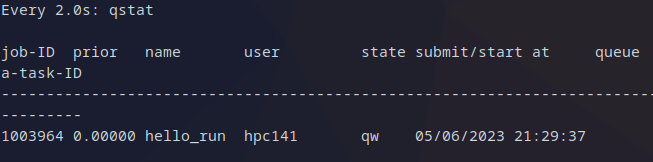
\includegraphics{hello_world_queue.png}
    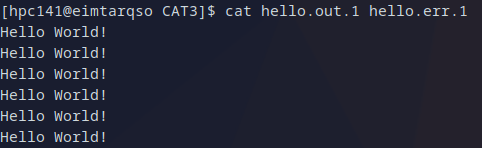
\includegraphics[scale=0.7]{hello_world_output.png}
    \caption*{Submit ./hello\_world to queue}
    \label{fig:1}
\end{figure}

With the provided SGE script we have:
\begin{itemize}
    \item \#\$ -pe orte 6: requests the allocation of 6 slots (or processes) for the job using the "orte" parallel environment (Open MPI).
    \item mpirun -np 6 ./hello executes the "hello" program with 6 processes using the mpirun command.
\end{itemize}
Each process prints "Hello World!" as output, as expected.

\begin{itemize}
  \item \textbf{What is the difference between the SGE option “-pe orte 6” and the MPI parameter “-np 6”?}
  ``-pe orte'' is an SGE option to request a parallel environment, with ``orte'' we give a specific environment within SGE to work with Open MPI and the number will be the slots to request. ``-np'', on the other hand, refers to the number of processes to launch by MPI.
  \item \textbf{What is the appropriate way of submitting to the queue the program with 2 processes (show your SGE code)?}
    \lstinputlisting[language=bash, label=lst:hello_np_2, caption={Submitting hello\_world.c with 2 MPI processes}]{hello_np2.sge}
\end{itemize}

\hypertarget{2}{%
\section{MPI Processes}\label{2}}

\subsection*{What is the result of the execution of the MPI program above (ranks.c) with 12 processes? Where did the ranks run? Why?}

\lstinputlisting[language=bash, label=lst:ranks12.sge, caption={Submitting ranks into the queue with 12 slots}]{ranks12.sge}
\begin{figure}[h!]
    \centering
    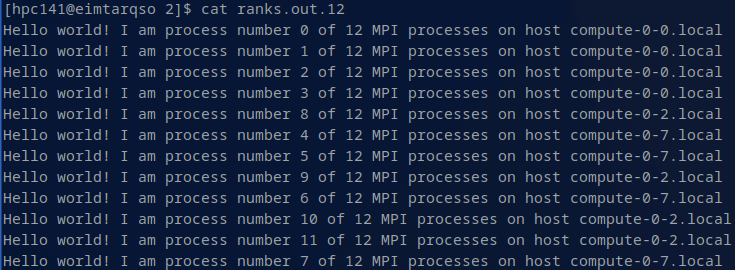
\includegraphics{ranks12.png}
    \caption*{./ranks submission to the queue with 12 slots}
    \label{fig:2}
\end{figure}

Processes with ranks 0 to 3 are running on the host "compute-0-0.local", processes with ranks 4, 5, 6, and 7 are running on the host "compute-0-7.local" and processes with ranks 8, 9, 10, and 11 are running on the host "compute-0-2.local".
The specific distribution of processes across different hosts depends on the configuration and availability of resources in the cluster and the scheduling algorithm of the resource manager.

This distribution may change depending on many factors (cluster's load, resources, etc.), for instance, a change in the SGE script to indicate to use 2 slots (Listing \ref{lst:ranks.sge}) may give the next results Fig. \ref{ranks12}.

\lstinputlisting[language=bash, linerange={7-9}, label=lst:ranks.sge, caption={Submitting ranks into the queue with 2 slots}]{ranks.sge}

\begin{figure}[h!]
    \centering
    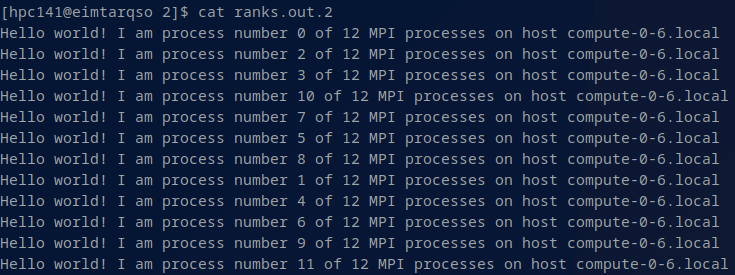
\includegraphics{ranks.png}
    \caption*{./ranks submission to the queue with 2 slots}
    \label{fig:2.2}
\end{figure}

The mismatch between the requested slots (2) and the number of processes (12) causes the processes to be oversubscribed on the available slots. As a result, the processes are all executed on "compute-0-6.local", since it is the only host available.

\hypertarget{3}{%
\section{Point to Point Communication}\label{3}}

\subsection*{With regard to deadlock.c:}

\begin{itemize}
  \item \textbf{Why does it deadlock?}
    Deadlock occurs when both processes (rank 0 and rank 1) execute the send operation first and then attempt to receive and wait for a message that will never arrive.
  \item \textbf{Can you describe how to prevent the deadlock? Provide and implementation of the previous program that prevents deadlocks. Attach the code, the execution output, and justify it.}
\end{itemize}

One possible solution is to use non-blocking communication with ``MPI\_Isend''(\ref{ref:MPI_Isend}), ``MPI\_Irecv''(\ref{ref:MPI_Irecv}) and ``MPI\_Wait''(\ref{ref:MPI_Wait}) functions.

\lstinputlisting[language=C, label=lst:ideadlock.c, caption={ideadlock.c: Use of non-blocking function for deadlock prevention}]{ideadlock.c}
\lstinputlisting[language=bash, label=lst:ideadlock.sge, caption={SGE script on deadlock prevention}]{ideadlock.sge}

\begin{figure}[h!]
    \centering
    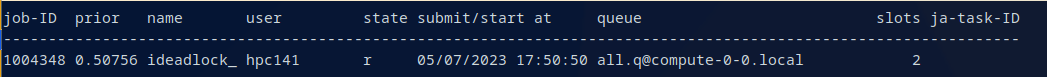
\includegraphics{ideadlock.png}
    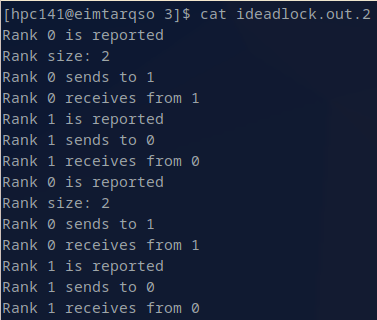
\includegraphics[scale=0.7]{ideadlock2.png}
    \caption*{./ideadlock submission to the queue with 2 slots}
    \label{fig:3}
\end{figure}

``MPI\_Isend'' starts a standard-mode, nonblocking send, ``MPI\_Irecv'' will start a nonblocking receive as well and ``MPI\_Waits'' waits for an MPI send or receive to complete.

\hypertarget{4}{%
\section{Matrix multiplication}\label{4}}

\subsection*{Using the code in matrixmul template.c, implement a program, where rank \#0 distributes a matrix multiply operation to the rest of ranks.}

\lstinputlisting[language=C, label=lst:matrixmul.c, caption={Matrix multiply operation across rest of ranks}]{matrixmul.c}

\begin{itemize}
    \item \textbf{Run your code with 8 processes (one producer and seven consumers).}
    \lstinputlisting[language=bash, label=lst:matrixmul.sge, caption={SGE script for matrixmul}]{matrixmul.sge}
    \begin{figure}[h!]
        \centering
        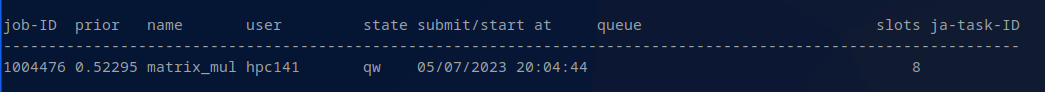
\includegraphics{matrixmul.png}
        \caption*{Sending code into queue}
        \label{fig:4}
    \end{figure}

    \item \textbf{Briefly explain your code.}\\
    This code demonstrates a parallel matrix multiplication using MPI (Message Passing Interface).\\
    If the rank is 0 (the producer), it initializes matrices A and B with some values. Then, the producer sends data to worker tasks by dividing the workload.\\
    It calculates the number of rows each worker will process based on the rank and the total number of ranks.
    Sends the offset (starting row index), number of rows, matrix A, and matrix B to each worker using MPI\_Send.\\
    After sending the data, the producer receives the results from each worker with MPI\_Recv.\\
    For the workers (with rank > 0), each receives the offset, number of rows and the matrices using MPI\_Recv and performs the matrix multiplication for its assigned rows of matrix A (calculated with offset) and matrix B (in full), and stores the result in matrix C.

    \item \textbf{Attach an screenshot of the execution of the prints given in the template.}
    \begin{figure}[h!]
        \centering
        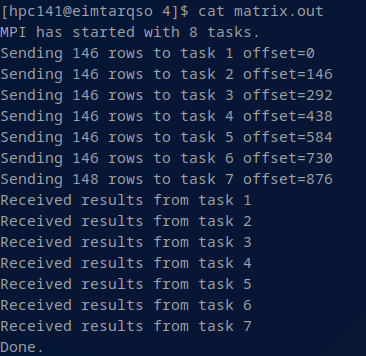
\includegraphics[scale=0.7]{matrixmul_exec.png}
        \caption*{Execution of the ./matrixmul program into the queue}
        \label{fig:4.1}
    \end{figure}
\end{itemize}

\hypertarget{5}{%
\section{Numerical Integration}\label{5}}

\subsection*{Implement a parallel version of trapezoid.c using MPI. The serial code provided in trapezoid.c uses the fragment function, which can be useful for your implementation.}

\lstinputlisting[language=C, label=lst:trapezoid_parallel.c, caption={Parallel version of trapezoid.c}]{trapezoid_parallel.c}
\begin{itemize}
    \item \textbf{Check that your results are equal to the serial version's results.}
    First execution of this exercise was naive and did not take into account a 60 min. timeout so after a first execution the output file was empty:
    \begin{figure}[h!]
        \centering
        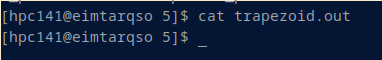
\includegraphics[scale=0.7]{trapezoid_serial_bad.png}
        \caption*{Execution of the serial verion of trapezoid.c in the queue}
        \label{fig:5}
    \end{figure}
    In order to avoid this caveat, the serial trapezoid program was edited by reducing its ``n'' param in order of 5 [\ref{lst:trapezoid_scratch}].
    \lstinputlisting[language=C, linerange={27-29}, label=lst:trapezoid_scratch, caption={Trapezoid edit ``n''}]{trapezoid.c}
    With this change we can see some results in the output file after seding the program to the queue [\ref{lst:trapezoid.sge}] [\ref{fig:5.1}].
    \lstinputlisting[language=C, label=lst:trapezoid.sge, caption={SGE script for serial trapezoid}]{trapezoid.sge}
    \begin{figure}[h!]
        \centering
        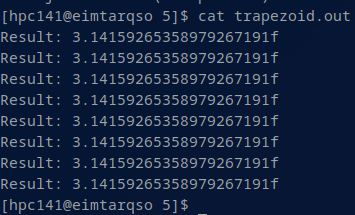
\includegraphics[scale=0.7]{trapezoid_serial_good.png}
        \caption*{Execution of the corrected serial verion of trapezoid.c in the queue}
        \label{fig:5.1}
    \end{figure}
    When we compare this results with the parallel version we see they are the same [\ref{fig:5.2}].
    \begin{figure}[h!]
        \centering
        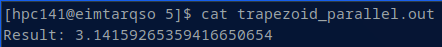
\includegraphics[scale=0.7]{trapezoid.png}
        \caption*{Execution of parallel verion of trapezoid.c in the queue}
        \label{fig:5.2}
    \end{figure}
    \item \textbf{Explain your design decisions, paying special attention to the MPI calls.}
    For this version we have several MPI calls

    \begin{itemize}
        \item MPI\_Init: Initializes the MPI environment as we saw erarlier [\ref{ref:init}].
        \item MPI\_Comm\_rank and MPI\_Comm\_size also initializes the MPI environment by determining a rank of the processes and a size associated to the communicator group. This is needed for the processes to communicate [\ref{ref:comm_rank}, \ref{ref:comm_size}]
        \item MPI\_Reduce: After the computation of the local fragment this function reduces the local results into a total result. ``MPI\_SUM'' will calculate the sum of all locals across processes [\ref{ref:reduce}].
        \item MPI\_Finalize: Terminates the execution environment [\ref{ref:MPI_Finalize}].
    \end{itemize}
    With these MPI calls we can divide the computation among the processes. Each process is assigned a local range to compute its own fragment of the integral. The workload is distributed evenly among the processes (local\_n = n / size) where ``n'' is the total number of fragments.

\end{itemize}


\hypertarget{6}{%
\section{MPI + OpenMP}\label{6}}

\subsection*{With regard to “trapezoid.c”:}
\begin{itemize}
    \item \textbf{Provide a MPI+OpenMP implementation of the code.}
    \lstinputlisting[language=C, label=lst:trapezoid_parallel_openmp.c, caption={MPI+OpenMP implementation}]{trapezoid_parallel_openmp.c}
    \lstinputlisting[language=bash, label=lst:trapezoid_parallel_openmp.sge, caption={Base SGE script}]{trapezoid_parallel_openmp.sge}
    \lstinputlisting[language=bash, label=lst:run.sh, caption={run.sh to build SGE scripts}]{run.sh}
    \item \textbf{Explain your design decisions (especially those related to \#pragma).}\\
    The code is basically the same as before (trapezoid with parallel implementation) but a new pragma sentence was added in order to make use of OpenMP.\\
    ``\#pragma omp parallel for'' is chosen to parallelize the ``for'' loop across threads. ``reduction(+:est)'' indicates the variable ``est'' needs to be reduced accross all threads with addition operation.
    \lstinputlisting[language=C, linerange={16-17}, label=lst:pragma, caption={Pragma added in for loop}]{trapezoid_parallel_openmp.c}
    This adding allows the program to parallelize the for loop and distribute the work across nodes with the parallel implementation in previous exercise.
    \item \textbf{Study the performance with different threads/processes configuration, and compare it to the only MPI version.}\\
    With the script \ref{lst:trapezoid_parallel_openmp.sge} we are able to store the execution times of each execution of the program in the queue, in Table \ref{tab:mpi-omp} we leave the results of each.
\end{itemize}

\begin{table}[]
    \centering
\begin{tabular}{|r|l|l|l|l|}
\hline
\multicolumn{1}{|c|}{\#nodes} & \multicolumn{1}{c|}{1ppn} & \multicolumn{1}{c|}{2ppn} & \multicolumn{1}{c|}{3ppn} & \multicolumn{1}{c|}{4ppn} \\ \hline
1                            &      0.06                     &               0.08            &0.08                           & 0.09                           \\ \hline
2                            &        0.04                   &             0.07              &    0.07                       &    0.07                       \\ \hline
3                            &       0.03                    &              0.06             &   0.07                        &    0.09                       \\ \hline
4                            &         0.03                  &      0.06                     &   0.08                        & 0.08                           \\ \hline
5                            &    0.06                       & 0.07                           &   0.19                        & 0.12                           \\ \hline
6                            &      0.04                     & 0.19                           & 0.11                           & 0.13                           \\ \hline
7                            & 0.05                           & 0.09                           & 0.24                           & 0.14                           \\ \hline
8                            & 0.06                           & 0.10                           & 0.13                           & 0.18                           \\ \hline

\end{tabular}
\caption{Performance experiments for processes per node (ppn)}
\label{tab:mpi-omp}
\end{table}

\section{References}
\begin{enumerate}
    \item Open MPI. (2022). \textit{MPI\_Isend(3): Starts a nonblocking send}. Retrieved from \url{https://www.open-mpi.org/doc/v4.0/man3/MPI_Isend.3.php} \label{ref:MPI_Isend}
    \item Open MPI. (2023). \textit{MPI\_Irecv(3): Starts a nonblocking receive}. Retrieved from \url{https://www.open-mpi.org/doc/v4.1/man3/MPI_Irecv.3.php} \label{ref:MPI_Irecv}
    \item Open MPI. (2021). \textit{MPI\_Wait(3): Waits for an MPI request to complete}. Retrieved from \url{https://www.open-mpi.org/doc/v3.1/man3/MPI_Wait.3.php} \label{ref:MPI_Wait}
    \item Open MPI. (2022). \textit{MPI\_Finalize(3): Terminates MPI execution environment}. Retrieved from \url{https://www.open-mpi.org/doc/v4.0/man3/MPI_Finalize.3.php} \label{ref:MPI_Finalize}
    \item Open MPI. (2023). \textit{MPI\_Reduce(3): Reduces values on all processes in a communicator}. Retrieved from \url{https://www.open-mpi.org/doc/v4.1/man3/MPI_Reduce.3.php} \label{ref:reduce}
    \item Open MPI. (2022). \textit{MPI\_Comm\_rank(3): Determines the rank of the calling process in the communicator}. Retrieved from \url{https://www.open-mpi.org/doc/v4.0/man3/MPI_Comm_rank.3.php} \label{ref:comm_rank}
    \item Open MPI. (2021). \textit{MPI\_Comm\_size(3): Determines the size of the group associated with a communicator}. Retrieved from \url{https://www.open-mpi.org/doc/v3.1/man3/MPI_Comm_size.3.php} \label{ref:comm_size}
    \item Open MPI. (2021). \textit{MPI\_Init(3): Initializes the MPI execution environment}. Retrieved from \url{https://www.open-mpi.org/doc/v3.1/man3/MPI_Init.3.php} \label{ref:init}

\end{enumerate}

\end{document}
